\documentclass[12pt, openany, a4paper]{book}
%\usepackage[spanish]{babel}
\usepackage[utf8]{inputenc}
\usepackage{graphicx}
\usepackage{subcaption}

\usepackage{wrapfig}

\usepackage{listings}
\usepackage[a4paper,top=3cm, bottom=3cm, inner=2.5cm, outer=2.5cm]{geometry}
\usepackage[colorlinks=true, 
linkcolor = black,
urlcolor  = blue,
citecolor = black,
anchorcolor = blue,
backref=page]{hyperref}
\usepackage{subcaption}
\usepackage{color}

\definecolor{codegreen}{rgb}{0,0.6,0}
\definecolor{codegray}{rgb}{0.5,0.5,0.5}
\definecolor{codepurple}{rgb}{0.58,0,0.82}
\definecolor{backcolour}{rgb}{1,1,1}

\lstset{frame=single,
	language=Python,
	aboveskip=3mm,
	belowskip=3mm,
	showstringspaces=false,
	columns=flexible,
	basicstyle={\small\ttfamily},
	numbers=none,
	backgroundcolor=\color{backcolour},   
	commentstyle=\color{codegreen},
	keywordstyle=\color{blue},
	numberstyle=\color{codepurple},
	stringstyle=\color{magenta},
	breaklines=true,
	breakatwhitespace=true,
	tabsize=3
}

\usepackage[acronym,nomain]{glossaries}
\newacronym{ai}{AI}{Artificial Intelligence}
\makeglossaries


\usepackage{tikz}
\usetikzlibrary{positioning}

\tikzset{basic/.style={draw,fill=blue!20,text width=1em,text badly centered}}
\tikzset{input/.style={basic,circle}}
\tikzset{weights/.style={basic,rectangle}}
\tikzset{functions/.style={basic,circle,fill=blue!10}}





%\usepackage{helvet}
\renewcommand{\familydefault}{\sfdefault}

\begin{document}
	%%%%%%% COVER %%%%%%%%
	\begin{titlepage}
	\begin{center}
		\vspace*{7.7mm}
		\includegraphics[width=0.4\linewidth]{images/logo}
		\vspace{6.5mm}
		
		\fontsize{15.5}{14}\selectfont ESCUELA TÉCNICA SUPERIOR DE INGENIERÍA DE TELECOMUNICACIÓN
		\vspace{13mm}
		
		\fontsize{14}{14}\selectfont GRADO EN INGENIERÍA EN SISTEMAS \\ DE TELECOMUNICACIONES
		
		\vspace{70pt}
		
		\fontfamily{lmss}\fontsize{15.7}{14}\selectfont \textbf{TRABAJO FIN DE GRADO}
		
		\vspace{25mm}
		\begin{huge}
			Deep Learning \\ on TensorFlow
		\end{huge}
		
		\vspace{25mm}
		
		\begin{large}
			Autor: Ignacio Condés Menchén

			Tutor: José María Cañas Plaza
		\end{large}
		\begin{normalsize}
			
			Curso académico 2017/2018
		\end{normalsize}
		\vspace{10mm}
	\end{center}
\end{titlepage}

\pagebreak
\thispagestyle{empty}
\vspace*{12cm}

\begin{flushright}
	\includegraphics[height=1.0cm]{images/CC-BY-SA}
	
	\vspace*{0.5cm}
	
	\copyright 2018 Ignacio Condés Menchén
	
	\vspace*{0.3cm}
	
	Esta obra está distribuida bajo la licencia de ``Reconocimiento-CompartirIgual 4.0 Internacional (CC-BY-SA 4.0)'' de Creative Commons.
	
	\vspace{0.2cm}
	
	Para ver una copia de esta licencia, visite
	http://creativecommons.org/licenses/by-sa/4.0/ o envíe una
	carta a Creative Commons, 171 Second Street, Suite 300,
	San Francisco, California 94105, USA.
\end{flushright}
	%%%%%%% INDEX, LISTS %%%%%%%%%
	\tableofcontents
	%\listoffigures
	%\listoftables
	
	%%%%%% SUMMARY %%%%%%%%%
	\chapter*{Summary}
	Nowadays, continuous improvements on Computer Science allow to address more complex tasks than traditionally. So, we can begin to artificially handle more \emph{human} tasks, which are performed on a more efficient way when the processing structure is modeled \emph{emulating human brain}. This field of study is covered by \emph{deep learning}, which particularly in the Computer Vision field makes the difference between a exhausting analysis of \emph{designed} features (which can be susceptible to environmental transformations or distortions), and \emph{automatically} extract abstract features, allowing a \emph{robust} operation, which can be executed on a  \emph{real time} manner.\\
	
	
	On the other hand \emph{robotics}, gradually more present in daily life, is more accessible, compatible and interoperable. This leads into a faster deployment of robots: not so long ago we only had huge, complex and not practical robots on production lines. Now we have autonomous vacuum cleaners perfectly able to clean our house and go back to its dock, at perfectly affordable prices for the vast majority of people.\\
	
	
	There is a really interesting \emph{synergy} between these two fields, which allow to combine the \emph{perception} skills that a \emph{deep learning} system can achieve, with the wide variety of physical \emph{responses} that a robot can perform.\\
	
	
	In this work, focused on introducing new \emph{deep learning} Computer Vision applications in the academics and research platform JdeRobot, three real-time components have been developed, making use of \emph{neural networks}: a \emph{digit classifier}, a generic \emph{object detector}, and a \emph{person following component}, which also incorporates a \emph{reactive behavioral to follow a specific person}. This is achieved combining an RGBD sensor, detection and facial analysis respective neural networks, and a robot equipped with wheels.	
	
	%%%%%% INTRODUCTION %%%%%%%%
	\chapter{Introduction}
This introductory chapter aims to present the general context which wraps this project, going in some depth inside \textbf{deep learning and robotics}. We will also amble along some of the latest advances and most useful current applications of the junction  these two fields. Lastly, we will situate this project on the previously described context. After this chapter, each key aspect of the work flow will be further explained.\\

\section{Robots}

Robotics applications can be really useful at daily tasks. These tasks are of greater interest when the behavioral of a robot tends to emulate the human one\footnote{\href{https://www.engadget.com/2018/01/08/new-sony-aibo-first-impressions/}{Some efforts are taken even into adopting the performance of human's best friend}}, with the advantage of no human beings exposed to a significant risk, or, in a less gloomy scenario, without human body physical limitations. This requires a polished (and somehow complex) behavioral, which is triggered by a certain input. At this point, we can find two main branches into robots, depending on the input source:
\begin{itemize}
	\item \textbf{Teleoperated robots:} this kind of robots are capable of perform certain actions, which are \textbf{remotely controlled by a human operator}. This application is the one with most weight on the hazardousness (\autoref{fig:1_pioneer}) \cite{chernobyl-robot} or precision \cite{teleop-surgery} factor. Thus, some advances are made nowadays improving the teleoperation function, implementing \emph{feedbacks} from the robot, such as haptic feedback \cite{teleop-haptic}, or VR (\emph{Virtual Reality}) sensation, to allow that person to sense the environment as if it was in front of her.	
	
	\item \textbf{Autonomous robots:} these robots are much more complex machines, as they are distinguished for implementing a response by itself, independently of any kind of remote operator. This is seeked on certain scenarios, where the time to perform an action or the cost of mantaining a critical link with a base, are factors with a considerable weight in the design \cite{ai-space}. This is the kind of robots that concern us on this work: the state-of-the-art techniques try to emulate \emph{human behavioral}(\autoref{fig:1_pepper}), so some actions can begin to be performed with a certain intelligence, as we will describe below.
\end{itemize}


	\begin{figure}[h]
		\centering
		\begin{subfigure}[b]{0.4\textwidth}
			\centering
			\includegraphics[width=0.8\linewidth]{images/pioneer_chernobyl}
			\caption{Pioneer robot, designed to perform hazardous teleoperated explorations in a deadly radioactive environment.}
			\label{fig:1_pioneer}
		\end{subfigure}
		\hfill
		\begin{subfigure}[b]{0.4\textwidth}
			\centering
			\includegraphics[width=0.8\linewidth]{images/pepper}
			\caption{Pepper, an autonomous humanoid capable of performing on board processing and reaction to external stimulus on a human way.}
			\label{fig:1_pepper}
		\end{subfigure}
		\caption{Robots of each described kind.}
		\label{fig:1_robots}
		
	\end{figure}

The important advances on the last decades on the image processing and audio recognition fields have impulsed the development of assistance systems, apart from critical machines as the previously described examples. \\

This way, several applications have arisen on people recognition and conversational behaviors, and it has been spread to everyday purposes, from personal assistants\footnote{\href{https://www.standard.co.uk/tech/google-smart-home-future-stay-a3868591.html}{Google Smart Home}}, to autonomous driving\footnote{\href{https://electrek.co/2018/06/18/what-tesla-autopilot-see-understand/}{Tesla Autopilot}}.\\

\section{Machine learning}
Almost every time, the mentioned behavioral is one or more reactive responses, triggered by a certain input (typically perceived by on-board sensors, among others). This raw data, which, is typically retrieved on a simple way (images, audio) is processed and mapped into a concrete response. At this point, we can bring up the key question: \emph{how do we process the raw input to obtain a suitable action for the current requirements, or needings?} The answer for that question is \textbf{machine learning}: the computer science field that pursues the capacity of machines to learn the suitable response to a previously unknown input. This is achieved by performing a training with a dataset of examples, which need to be properly formatted: the system has to previously know what to look for and evaluate, what is typically called \textbf{features}, and learn the proper parameters for an optimum output.\\

Generally, machine learning problems can be split into two types of response (\autoref{fig:1_class_vs_det}):

\begin{itemize}
	\item \textbf{Classification:} given a set of possible classes $\{c_1, c_2, ..., c_n\}$ to which an image $x_i$ can belong, we select the class $c_i$ where $x_i$ fits the best, given a set of features extracted from it.
	\item \textbf{Detection}: given an image $x_i$, we decide if we can find or not an object/region inside of it which fits into the searched type. In the affirmative case, we locate it (using a region or a bounding box).
\end{itemize}

\begin{figure}[h!]
	\centering
	\begin{subfigure}[h!]{0.6\textwidth}
		\includegraphics[width=\textwidth]{images/classification}
		\caption{Classification}
		\label{fig:1_classification}
	\end{subfigure}
	
	\qquad
	
	\begin{subfigure}[h!]{0.6\textwidth}
		\includegraphics[width=\textwidth]{images/detection}
		\caption{Detection}
		\label{fig:1_detection}			
	\end{subfigure}
	
	\caption{Functional difference between \textbf{classification} and \textbf{detection}.}
	\label{fig:1_class_vs_det}
\end{figure}

\section{Deep Learning}
\emph{Deep learning} is the piece of machine learning that is capable to \textbf{automatically learn the features that the system could use from primary data} (pixels on images, samples on audio, words in text processing, etc.).\\
\subsection{Neural Networks}
This has turned deep learning into the cornerstone of current applications of \emph{AI}, which don't need complex dataset with a lot of preprocessing (that require important human effort) anymore. That simplicity is achieved through the use of \emph{Neural Networks}. A Neural Network is the representation of an algebraic algorithm which implements non-linear calculus models \cite{dl-nature}. It is composed by several processing \textbf{layers}, which are made up of \emph{perceptrons}, that are generally called \textbf{neurons}. This is because these neural structures \textbf{emulate the human brain}, formed by a huge set of interconnected neurons, which are disposed on the already mentioned layers (\autoref{fig:1_neural_network}).\\

\begin{figure}[htpb]
	\centering
	\includegraphics[width=5cm]{images/neural_network}
	\caption{Structure of a Neural Network}
	\label{fig:1_neural_network}
\end{figure}

First approaches to neural networks, according to \cite{nn-history} were developed on the 50s-60s decades. This was when the computational potential allowed to develop on a real machine the first modeling of the way it was believed that a brain neuron works, which was inspired by electrical circuits. These experiments \cite{first-neuron} were performed by the neurophysiologist W. McCulloch and the mathematician W. Pitts. Later, in 1949, Donald Hebb \cite{hebb} observed that the synaptic path between two neurons is reinforced (its efficiency rises up) every time it is used. This introduced the concept of \textbf{training} on a neural network.

\subsection{Processing unit: the perceptron (neuron)}
\begin{figure}[h]
	\centering
	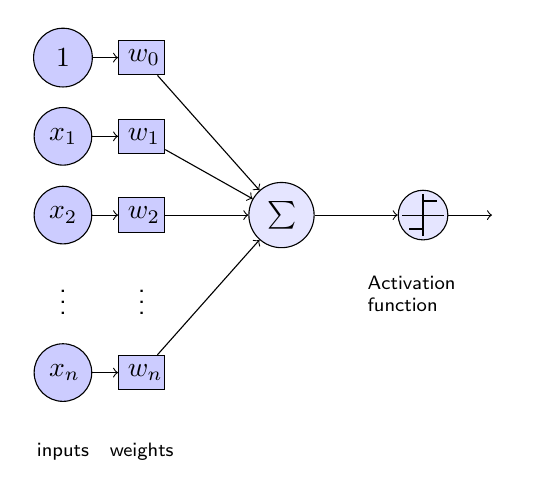
\begin{tikzpicture}
	\node[functions] (center) {};
	\node[below of=center,font=\scriptsize,text width=4em] {Activation function};
	\draw[thick] (0.5em,0.5em) -- (0,0.5em) -- (0,-0.5em) -- (-0.5em,-0.5em);
	\draw (0em,0.75em) -- (0em,-0.75em);
	\draw (0.75em,0em) -- (-0.75em,0em);
	\node[right of=center] (right) {};
	\path[draw,->] (center) -- (right);
	\node[functions,left=3em of center] (left) {$\sum$};
	\path[draw,->] (left) -- (center);
	\node[weights,left=3em of left] (2) {$w_2$} -- (2) node[input,left of=2] (l2) {$x_2$};
	\path[draw,->] (l2) -- (2);
	\path[draw,->] (2) -- (left);
	\node[below of=2] (dots) {$\vdots$} -- (dots) node[left of=dots] (ldots) {$\vdots$};
	\node[weights,below of=dots] (n) {$w_n$} -- (n) node[input,left of=n] (ln) {$x_n$};
	\path[draw,->] (ln) -- (n);
	\path[draw,->] (n) -- (left);
	\node[weights,above of=2] (1) {$w_1$} -- (1) node[input,left of=1] (l1) {$x_1$};
	\path[draw,->] (l1) -- (1);
	\path[draw,->] (1) -- (left);
	\node[weights,above of=1] (0) {$w_0$} -- (0) node[input,left of=0] (l0) {$1$};
	\path[draw,->] (l0) -- (0);
	\path[draw,->] (0) -- (left);
	\node[below of=ln,font=\scriptsize] {inputs};
	\node[below of=n,font=\scriptsize] {weights};
	\end{tikzpicture}
	\caption{Diagram of a perceptron/neuron}
	\label{fig:1_perceptron}
\end{figure}


Every neuron is composed by an structured schema:
\begin{enumerate}
	\item \emph{Inputs}: the data which come into the neuron. It might come from the main stimulus, or from another neuron (as the output of the previous layer)
	\item \emph{Weights}: the tuned parameters of the network. They represent the importance given to each feature on that singular neural unit. The weight $w_n$ multiplied $x_n$ times results on the contribution of the feature $n$ in the current neuron. 
	\item \emph{Sum}: the product of all the inputs with their suitable weight come into a sum operation\footnote{We consider $w_0$ as the product to the constant input $1$, as the intercept term (a constant always present independently of the current input).}, to \textbf{build a total linear response:} $ z = \sum_{i=0}^{n}x_i \cdot w_i$\footnote{There is also a summation bias term on each neuron, $b_i$, but it is ignored here for the sake of simplicity, as the weights are more representative with respect to the input.}.
	\item \emph{Activation function}: this is an important part of a neural network as, until this moment, all the numerical computations we have performed were just linear operations. If we keep the output of the neuron being a linear function of the input, we will lose the effect of having more than 1 layer, as really the total result of all the network is a linear function of the first input, so we could simplify all the network down to one single neuron. \\
	
	For this reason, we use a \textbf{non-linear activation function}, which maps the linear combination computed by the sum, into the $[0,1]$ interval, on a non-linear function. A typical function is the one called \emph{ReLU} (REctified Linear Unit) \cite{relu}, which follows the formula:
	\begin{equation}
		g(z) = max(0, z)
		\label{eqn:1_relu}
	\end{equation}
	
	\item \emph{Output}: when the activation function has been computed, it is forward-propagated to the output, or to the neurons belonging to the next layer. As it has been said, it is mapped into the $[0, 1]$ interval, so it can be seen as the importance that particular feature will have on the next neuron: if it takes nearly zero values, the next neuron will be poorly stimulated. There lies the meaning of the name of the previous component: \emph{activation function}.
\end{enumerate}

\subsection{Deep Neural Networks}
The fact of having more than one layer gives to the network the concept of \emph{depth}. This opens the door to a vast set of possibilities, as \textbf{it allows us to perform deep learning with neural networks: Deep Neural Networks}. This can be achieved, as we can see on \autoref{fig:1_deep_nn}, by introducing a new kind of layer, where all the new neurons are connected to every single neuron of the previous one.\\
This is typically called a \textbf{fully connected layer}, and the fact of relating every single activation from the previous layer with a set of tunable weights on each neuron allows to rapidly find common patterns followed by features seen on one of the analyzed scenarios (e.g. syntactical relationships between several kinds of words in language processing, or finding edges or shapes on image detection/classification).

\begin{figure}[h]
	\centering
	\includegraphics[width=0.9\linewidth]{images/deep_neural_network}
	\caption{Evolution to a \textbf{deep} neural network.}
	\label{fig:1_deep_nn}
\end{figure}

\subsection{Convolutional Neural Networks (\emph{CNNs})}

Finally, this leads us to the last concept we will study on this dissertation. As we have said before, we can connect a big set of neurons between themselves to extract more abstract and complex features, of increasing interest with the number of neurons and layers.\\
 
If we aim to apply this processing to images, we have to take into account that, if we want to input an image into a neural network, each pixel has to be taken as an input, and also the fact that an RGB image is composed of 3 channels (1 channel per color), so, for an image with a dimensions of $m$ pixels wide and $n$ pixels high, we will need $m\cdot n \cdot 3$ input neurons. Besides this considerable number, we will have to take into account the neurons resulting on the additional deeper layers that we will add to have an high enough abstraction level for our application. This drives to absurd numbers of simultaneous neurons working, that are difficultly handable during a feed-forward execution, but absolutely unfeasible on a training process. An additional problem can be a moving object/region on the image: we must be capable to detect the shape of a car on the right side of the image, or in the left one.\\

We can solve both problems simultaneously with an easy procedure: we will not process the entire image at one time. Instead of that \textbf{we will perform a convolution operation between the inputs of our network, and different regions of the image}. This will output \emph{activation maps}, which symbolize the response of that portion of the image to the input weigths. This can be performed, as we have said before, a few times to obtain features with a higher degree of abstraction. As we want to keep the computational complexity low, we can alternate these layers with \textbf{pooling layers}, which subsample the resulting maps, to keep it simple (if we keep only 1 of each 3 pixels of an activation map, selecting it carefully to retain the maximum information, we can reduce the number of necessary neurons on the next layer on a factor of $\frac{1}{3} \cdot \frac{1}{3} = \frac{1}{9}$). This is reflected on \autoref{fig:1_cnn}, where the process of convolution-pooling can be repeated a few times, and then the result (which should not have considerably big dimensions) are inputted into a fully connected layers, to extract and handle the relations between the features and the possible classes (on a classification scenario).

\begin{figure}[h]
	\centering
	\includegraphics[width=0.9\linewidth]{images/cnn}
	\caption{Schematic of a CNN.}
	\label{fig:1_cnn}
\end{figure}

\section{Deep Learning on JdeRobot}

So, as we have been describing, Deep Learning can be of a great interest on the image processing field, as it allows to implement an easy and really robust AI algorithm.\\

JdeRobot\footnote{\url{https://jderobot.org}} is a software development suite, developed from inside this University, and among all the developed software/investigation inside it, we can find some interesting programs/projects for our purposes:

\begin{itemize}
	\item \texttt{Detection Suite}\footnote{\url{https://github.com/JdeRobot/dl-DetectionSuite}}: it is a C++ application, suitable to load/benchmark \textbf{detection} models, against different databases. It is also capable, through a Python$\rightarrow$C++ interface, to load TensorFlow/Keras models as well.
	
	\begin{figure}[h]
		\centering
		\includegraphics[width=4in]{images/detection_suite_depth}
		\caption{\texttt{DetectionSuite} on action.}
		\label{fig:1_detectionsuite}
	\end{figure}

	\item Final project of David Pascual \cite{dpascualhe} and Nuria Oyaga \cite{noyaga}: a further study of Deep Learning, applied on Python (Keras and Caffe frameworks, respectively) to \textbf{digit classification} implementing a CNN as it has been seen.
	\begin{figure}[h]
		\centering
		\includegraphics[width=4in]{images/digitclassifier}
		\caption{\texttt{DigitClassifier} working.}
		\label{fig:1_digitclassifier}
	\end{figure}
	
	\item MsC project of Marcos Pieras \cite{marcospieras}: On this interesting thesis, an application implementing two neural networks (as we will do) has been developed. One of them allows us to \textbf{detect} people on an image, and the other one (a siamese network, as we will describe later) can track features of each person, to keep every detected individual identified on a surveillance image system (and possibly trace the route followed by each person).
	\begin{figure}[h]
		\centering
		\includegraphics[width=4in]{images/people_tracker}
		\caption{\texttt{PeopleTracker} working.}
		\label{fig:1_people_tracker}
	\end{figure}
	
\end{itemize}

In conclusion, as we have been mentioned, and we have already taken a glance on the possible applications, Deep Learning can make such a brilliant tandem along with a reactive behavioral, as we will demonstrate on this project.\\

\begin{center}
	\textbf{Robotics + deep learning rock!}
\end{center}



	
	
	%%%%%% OBJECTIVES %%%%%%
	\chapter{Objectives and Methodology}

\section{Objectives}

Keeping all of this in mind, we can now bring up the main purpose of this investigation labor, which is to generate a behavioral focused on tracking and actively following a person, making use of a robot. This internal process of transformation of the stimuli into a movement will be accomplished using \textbf{convolutional neural networks}.\\

With all this in mind, the objective of the present work has been to get a little further on \textbf{deep learning applied to robotics}, developing two consecutive components, each one functionally focused on a purpose. They will be introduced right below.
	\begin{itemize}
		\item \textit{Detection:} As it will be described on the suitable chapter, we will build a component (\texttt{Object Detector}) which implements \textbf{a generic object detection algorithm} on an incoming video stream. This component will be ready to work in \emph{real time}.
		
		As it can be inferred, it will not provide a response \textit{per se}. Its visible output will be to draw \emph{bounding boxes} surrounding each detected object, indicating as well the class where that particular object belongs (person, airplane, dog, etc.), and its score (confidence in \%).
		
		\item \textit{Tracking and following:} As we want to implement a following behavioral, our main objective here is to \textbf{identify and track} the person to follow, which will semantically be called \emph{mom}. The component that comprehends the previous detection behavioral and this new one will be named \texttt{Follow Person}. The great advantage here is the strength a CNN can achieve under variable light conditions. That makes this technique perfectly suitable to command physical actuators on a robot.
		
		We will make use of the detected people (with the technique followed on the previously described node and constraining the result to only retain people detection), and look for the face of each one of them. Later, we will make use of another neural network technique, called a \emph{siamese network} (it will be properly explained later) to identify them. It will allow us to find \emph{mom}, in case it is being seen by the camera, and command a proper response to the robot with the objective of following \emph{mom}.
	\end{itemize}

As we have said before, these two nodes/components are successive. Thus, they will share an important part of the global objectives.\\

We will start breaking down the common objectives between both applications, into three functional blocks:

\begin{itemize}
	\item \textit{Design:} both milestones have been preceded by a first \textbf{documentation} phase. While the theoretical base was learned and achieved, some papers and examples were investigated. We will go some deeper in each section.
	
	Later, a more specific design phase will be to specify the structure of the nodes.
	From now on, we will have to perform several tasks simultaneously:
	\begin{itemize}
		\item Grabbing the incoming image(s) from the sensor(s).
		\item Processing the image(s).
		\item Properly update the GUI (\textit{Graphical User Interface}) with the image(s) and the outputs of the processing.
		\item \textit{Only on the following node:} send the computed response order to the actuators.
	\end{itemize}
	%
	These tasks should follow an \emph{asynchronous schema} every time, to avoid blocks between tasks, and taking advantage of some shared memory to exchange inputs/outputs. Besides, this allows us to have a custom iteration period for each task: we shouldn't have to wait until the neural network finishes feed-forwarding the image to refresh the \emph{GUI}. On a high level structure, it could follow the schema on the \autoref{fig:2_tasks}.
	
	\begin{figure}[h]
		\centering
		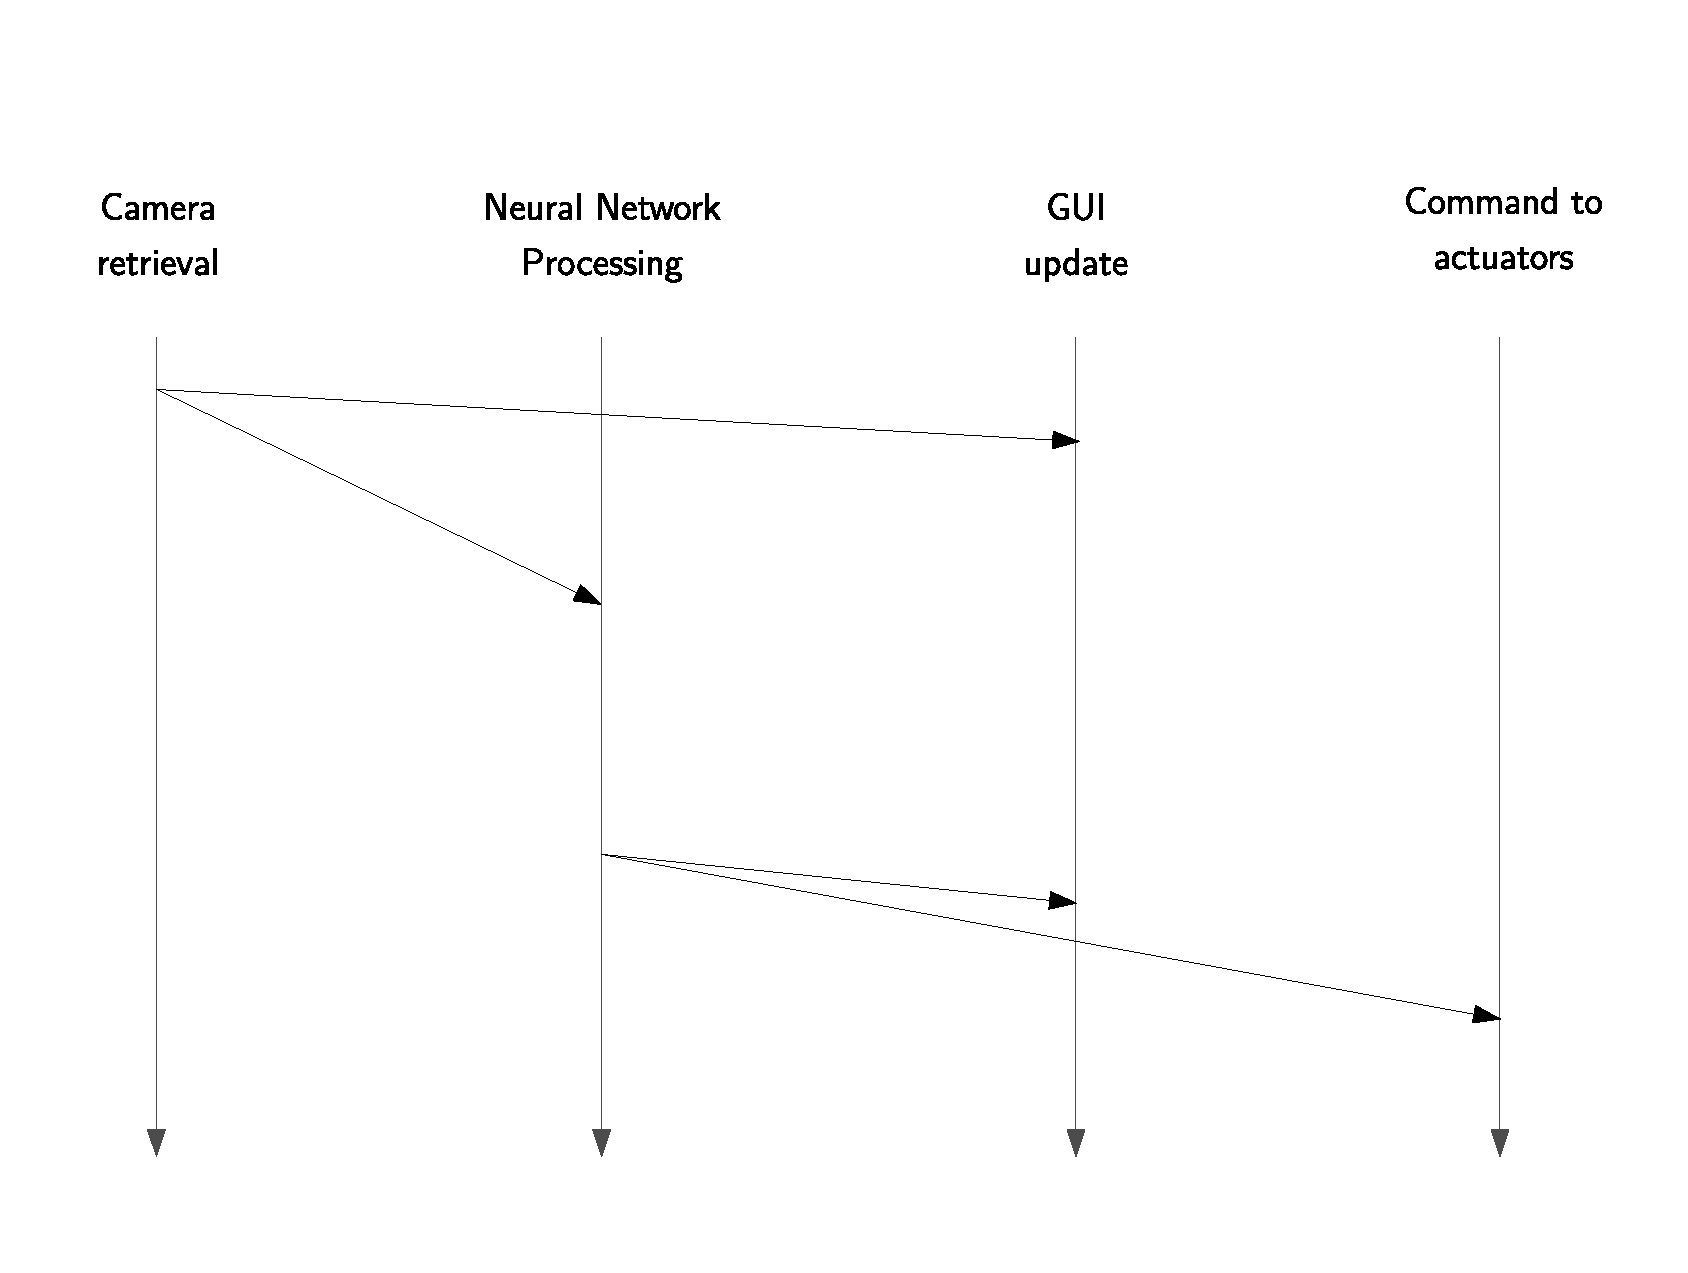
\includegraphics[width=3in]{images/tasks_threads}
		\caption{Parallel tasks to perform, and data exchange between them.}
		\label{fig:2_tasks}
	\end{figure}
	
	\item \textit{Implementation:} the next and most time consuming objective is to \textbf{develop both components}. The advantage is, once again, that both components are successive. This makes code reutilization a very interesting move, as we will only need to perform a language-friendly additions (on a simple way, thanks to \textit{Object Oriented Programming})) to the \texttt{Object Detector} code to implement the \texttt{Follow Person} features (depth images support, computing and commanding movements to the motors, among others). Details will be described on the appropriate section.
	
	\item \textit{Experimentation\footnote{\textit{"In theory, theory and practice are the same. In practice, they are not."}, Y. Berra}:} these nodes have a very strong tunability component (from neural network parameters to movement factors in the commands for the motors, stopping over describing all the desired behavior that the following algorithm has to adopt in several situations that it has to be capable of handling).
	
\end{itemize}

Finally, we will briefly highlight the \textbf{personal} objectives we have pursued on this project. As this has been developed along a whole year, and on a relatively abstract field as \emph{deep learning} is, a level of rigour has been necessary to accomplish satisfactory results. This provides a novice investigator the opportunity to learn about the phases and development process on a much more professional way than a homework task. \\

In addition, this project has allowed an interested person in \emph{deep learning} to learn about a cornucopia of concepts and experience. Later, when it was decided to evolve towards creating a reactive behavioral, it was motivating to make the most of a possible synergy between two different fields of knowledge, as \emph{deep learning} and \emph{robotics} are. It has to be remarked that the implementation of the development has always been possible, so it has been easy where there was more work to do in every moment.

\section{Methodology}
The workflow present on this project has been supported by weekly meetings.

MediaWiki

GitHub repo

Functional videos

	
	%%%%% INFRASTRUCTURE %%%%%
	\chapter{Infrastructure}

	This chapter is destined to a brief description of all the available hardware/software resources on which we will rely along the project.\\
 
\section{Hardware}
	\subsection{Sony EVI D100P camera}
	\label{sec:3_ptz}
		\begin{figure}[h]
			\centering
			\begin{subfigure}[h]{0.4\linewidth}
				\centering
				\includegraphics[width=1.6in]{images/ptz_front}
				\caption{Front side.}
			\end{subfigure}
			\qquad
			\begin{subfigure}[h]{0.4\linewidth}
				\centering
				\includegraphics[width=1.6in]{images/ptz_back}
				\caption{Back side.}
			\end{subfigure}
			\caption{Sony EVI D100P.}
			\label{fig:3_evi}
		\end{figure} 
		
		The first used hardware element is the Sony EVI D100P\footnote{\url{https://pro.sony/en_IN/products/ptz-network-cameras/evi-d100-d100p-pal-}}. It is a \emph{PTZ} cam (which stands for \emph{Pan Tilt Zoom}) which, originally thought and designed for videoconferences, is equipped with a bunch of precision servo motors. This allows it to be teleoperated, performing a soft and steady two-dimensional movement on demand:
		\begin{itemize}
			\item \emph{Pan:} horizontal movement. It can take values from $-100$ to $100$ degrees from the centered position. This movement can be performed at a certain speed, which can be set between $1$ and $24$.

			\item \emph{Tilt:} vertical movement. Its range goes from $-30$ to $30$, and the movement speed can be also varied between $1$ and $20$.
		\end{itemize}
		
		Something remarkable about this device is that it is bidirectional: we \textit{receive} images from its camera, and, at the same time, we \textit{send} it commands to move the motors.\\
		
		\begin{description}
			\item[Motors] 
			The low-level implementation of the movement commands is the \emph{VISCA} protocol, a proprietary solution from the manufacturer (Sony). It is received by the cam through a RS-232C (the traditional low-rate serial interface before USB spread), so we can connect it to a modern computer with a RS232-USB interface.
			
			However, the driver that controls this camera (\autoref{sec:3_evicam_driver}) does not offer support for a \emph{zoom} movement, but it is not very relevant for this application.\\
			
			\item[Video] 		As the video sensor is an analogue device, we need to convert its information to a digital format. We achieve this with a video capture device (\autoref{fig:3_dazzle}), which outputs digital video. This image flow is processed by a ROS driver (\autoref{sec:3_usb_cam}), that will be later explained.
			
			\begin{figure}[h]
				\centering
				\includegraphics[width=3in]{images/pinnacle_dazzle}
				\caption{Analogue-digital video converter (Pinnacle Dazzle).}
				\label{fig:3_dazzle}
			\end{figure}
			
			
		\end{description}

	
		We have to be careful on the movement commands (as it will be seen on \autoref{sec:follow_ptz}).\\

		This is the device we use on our experimental approach to the \emph{detection + robotic behavioral} node (\autoref{sec:follow_ptz}), where the only response is moving the camera.\\

	\subsection{Asus Xtion Pro Live}
		\label{sec:3_xtion}
		It is a RGBD (RGB + Depth) sensor, designed by Asus for interactive PC applications development purposes.

		\begin{figure}[h]
			\centering
			\includegraphics[width=0.4\linewidth]{images/xtion}
			\caption{Asus Xtion Pro Live. IR emitter (left), and RGB and IR lenses (right).}
			\label{fig:3_xtion}
		\end{figure}

		It counts on its left side with an IR (\emph{infrared}) light emitter, which radiates beams like a conventional light bulb (that's its function). On the right side, we can find two sensors:
		\begin{itemize}
			\item \emph{RGB sensor:} a regular digital camera, with a resolution up to 1280x1024 px.
			
			\item \emph{Depth sensor:} measures distance to objects by receiving the reflections of the IR beams that we have mentioned above. It maps, for each pixel, the distance to that reflection (in mm), stored as a 16-bit long value. Thus, we can obtain a depth image, with a resolution of 640x480 px (@ 30 fps).
		\end{itemize}

	We have used it as the visual source in the developed \emph{detection + robotic behavioral} node (\autoref{chap:followperson}).\\
		
	
	\subsection{Turtlebot 2 robot}

		\begin{figure}[h]
			\centering
			\begin{subfigure}[h]{0.4\linewidth}
				\includegraphics[width=1.9in]{images/real_turtlebot_1}
				\caption{Frontal view.}
				\label{fig:3_turtlebot_front}
			\end{subfigure}
			\begin{subfigure}[h]{0.4\linewidth}
				\includegraphics[width=2.2in]{images/real_turtlebot_2}
				\caption{Side view.}
				\label{fig:3_turtlebot_side}
			\end{subfigure}
			\caption{Turtlebot development kit.}
			\label{fig:3_turtlebot}
		\end{figure}
		
		It is a research robot, composed by a structure jointed to a Kobuki robot (mobile base)\footnote{\url{http://kobuki.yujinrobot.com/about2/}}. According to its technical specifications\footnote{\url{https://www.robotnik.es/web/wp-content/uploads/2014/04/TB_robot.pdf}}, it can reach speeds of $700 \ mm/s$ (on straight line), and $180\ deg/s$ (turning). Into the attached structure, we can find mounted an Asus Xtion sensor.\\
	
		The user has the capability of connecting each of these devices via USB to the laptop, and place it at the top platform of the robot. From there, the computer can run the algorithm and command the movements. Every component can be handled with the respective ROS driver (which will be described later).
		
		The Turtlebot platform has been our main actuation platform for the developed \emph{detection + robotic behavioral} application (\autoref{chap:followperson}).\\
			

\section{Python}
	According to the official definition from \cite{python}, Python is \textit{an interpreted, object-oriented, high-level programming language with dynamic semantics}. It was created in 1991 by Guido van Rossum. However, due to the increasing growth of \emph{Machine Learning} that happened the last two decades, it has become the most popular language for this purpose. As it focus on \emph{easiness}, its duck typing\footnote{This refers to Python guessing about your code, coming from the phrase \textit{''if it looks like a duck and sounds like a duck, chances are it's a duck."}} and its strong Object Orientation (everything can be treated as an object on this language) are a big ace up the sleeve in comparison to other languages and alternatives. In the programming point of view, it is a very interesting feature, as it facilitates features as sharing memory, abstract processes, and much more.
	
	And it is \textit{Open Source}, so it is always under community improvements, and there are a vast number of useful third party libraries, which often are pretty easily deployable onto your code.\\
	
	All these points make this language a really potential candidate for the applications to develop (and that's precisely the reason that explains its  growth on the software market).\\
	
	Python is an \emph{interpreted} language, which means that its sentences are projected on another program (the CPython interpreter, which executes them), and not directly by the processing hardware (CPU/GPU). This can be a handicap, as it makes the code execution much slower, in comparison with standard \emph{compiled} languages, which are run directly as processes, and grabbed by the computer hardware for its execution (as C, C++, Picky, etc.).\\
	
	For our target, we have used Python on its version $2.7$. Although it is a relatively old version of the language, it is necessary to mantain the compatibility with ROS Kinetic distribution  (\autoref{sec:3_ros}) bindings, which have not still taken the leap to the newest major version ($3.x$) on Python.\\
	


\section{ROS robotics framework}
	\label{sec:3_ros}
	\emph{ROS} (Robot Operating System) is \textit{an open-source, meta-operating system for your robot}, maintained by the \emph{OSRF} (Open Source Robotics Foundation) \cite{ros-intro}. It is a framework that provides a distributed, easily-scalable environment of \emph{nodes}. These nodes are programs which are independently on the computer (or distributed over a network), so they can perform individual tasks. However, they can communicate between themselves on a synchronous way (over \emph{services}, implementing a client-server role system between nodes), or on an asynchronous way, via \textit{topics}. These topics, which rely on a standard TCP/UDP communication between sockets via the \texttt{loopback} interface, are intended for an unidirectional, streaming communication, where a node can take roles: \emph{publisher} (if it is writing data inside the topic), or \emph{subscriber} (if it is reading the data that publishers are broadcasting into the topic). The data stream through the topic is not unrestricted. It must follow a ROS specific syntax, the \emph{Message} type, which is strictly defined for the communication purpose (geometry, sensoring, etc.).\\
	
	For our project we have used the 2016 \textit{LTS} (Long Term Support) version, called \textit{Kinetic Kame}\footnote{\url{http://wiki.ros.org/kinetic}}. This is the version bundled on the installation of JdeRobot\footnote{\url{https://jderobot.org/Installation}}, which offers a full compatibility with it.\\
	

	\begin{figure}[h]
		\begin{lstlisting}
...
import rospy
from std_msgs.msg import String
...
rospy.init_node('listener')              # Starting the node entity.
rospy.Subscriber('chatter', String)      # Instantiation of the topic subscriber.
rospy.spin()                             # 'Infinite loop' listening to the topic.
...
		\end{lstlisting}
		\caption{Simple stablishment of a listener node through \texttt{rospy} (code from \cite{listener-rospy}).}
		\label{fig:3_rospy_listener}
	\end{figure}
	
	ROS provides libraries and bindings for C++, Lisp, and \textit{Python} (\texttt{rospy}). They allow to really easily set up a topic between two or more programs, which will be seen as ROS nodes. However, this topic communication will be abstracted on our project by the \texttt{comm} library, as it will be seen on \autoref{sec:3_comm}.\\
	
	ROS also provides a Debian package, called \texttt{rosbash}, which allows to, in a very handy way, manage nodes and packages from a standard \texttt{bash} shell. The most remarkable feature for us is the command \texttt{roslaunch}, that launches a ROS node with a certain specific settings, configurable via a \texttt{.launch} file (which follows a XML formatting). An example for the file structure can be found on \autoref{fig:3_launch_file}.\\
	
	\subsection{usb\_cam driver}
	\label{sec:3_usb_cam}
		It is a ROS driver that creates a topic and publishes into it the digital video data incoming from a USB camera, into the topic \texttt{/usb\_cam/image\_raw}.\\
		
		This driver has been used on some experiments about the \emph{detection + robotic behavioral} application (\autoref{sec:follow_ptz}), with the purpose of retrieving images from the Sony EVI D100P camera (\autoref{fig:3_evi}). A custom configuration file\footnote{\url{https://github.com/RoboticsURJC-students/2017-tfg-nacho\_condes/blob/master/resources/usb\_cam-test.launch}} is required. We can have a glance on that configuration file on \autoref{fig:3_launch_file}.\\
		
		\begin{figure}[h]
			\centering
			\includegraphics[width=5in]{images/usb_cam_test}
			\caption{Example of \texttt{usb\_cam-test.launch} configuration file for a ROS node.}
			\label{fig:3_launch_file}
		\end{figure}
		\begin{center}
			Usage: \texttt{roslaunch usb\_cam-test.launch}
		\end{center}

	\subsection{openni2\_launch driver}
	
		The ROS binding at \cite{openni2-doc} provides the launch files for the \texttt{rgbd\_launch} node. This node publishes on several topics the RGB+D images provided by the Asus Xtion (\autoref{fig:3_xtion}).\\
		

		
		As it can be seen on \autoref{fig:3_xtion}, both sensors (RGB and infrared) can't physically be in the same place, so there is a little discrepancy between both computed image:
		
		\begin{figure}[h!]
			\centering
			\begin{subfigure}[h]{0.4\linewidth}
				\centering
				\includegraphics[width=2.7in]{images/rgb_before}
				\caption{RGB image.}
				\label{fig:3_rgb_bef_reg}
			\end{subfigure}
			\hfill
			\begin{subfigure}[h]{0.4\linewidth}
				\centering
				\includegraphics[width=2.7in]{images/depth_before}
				\caption{Depth image.}
				\label{fig:3_depth_bef_reg}
			\end{subfigure}
			
			\caption{Both raw (before registration) images sensed by the Xtion cameras.}
			\label{fig:3_bef_reg}
		\end{figure}
		
		With the goal of palliating this disparity, a process called \emph{registration} is executed for every new incoming depth image. It consists of a projection of the depth pixels into the RGB image, trying to align on an optimum way each depth pixel with its counterpart on the RGB image. We can observe that this can cancel to a certain point the difference between both images (\autoref{fig:3_disparities_comp}).
		
		\begin{figure}[h]
			\begin{subfigure}[h]{0.4\linewidth}
				\centering
				\includegraphics[width=2.7in]{images/disparity_before}
				\caption{Before registration.}
				\label{fig:3_disparity_bef_reg}
			\end{subfigure}
			\hfill
			\begin{subfigure}[h!]{0.4\linewidth}
				\centering
				\includegraphics[width=2.7in]{images/disparity_after}
				\caption{After registration.}
				\label{fig:3_disparity_aft_reg}
			\end{subfigure}
			\caption{Comparison between the disparities, before and after the registration process.}
			\label{fig:3_disparities_comp}
		\end{figure}
		
		If we compare the new disparity (\autoref{fig:3_disparity_aft_reg}) with the previous one (\autoref{fig:3_disparity_bef_reg}), we can realize that now the RGB and Depth images are aligned on an improved way, as if both sensors were on the same place, or much closer at least. So, from now on, we will call \emph{depth image} to the registered version of the depth map, as the unregistered image is not useful anymore.\\
		
		The open source driver working behind this binding is called OpenNI\footnote{\url{https://structure.io/openni}} (\emph{Open Natural Interaction}). It was originally written by the Kinect developer company PrimeSense (which designed the Xtion device beside Asus).\\
		
		In summary, this interface allows to perform both processes involved into handling this device (image grabbing and depth registration). It has been used on the {detection + robotic behavioral} application (\autoref{chap:followperson}). It will connect the Xtion sensor to it, providing the real time imaging through the corresponding topic.\\
		
		\begin{center}
			Usage: \texttt{roslaunch openni2\_launch openni2.launch}
		\end{center}

	\subsection{kobuki\_node package}
		This ROS package contains a bunch of launch files. Among them there is the one we have used: \texttt{minimal.launch}, which starts the \emph{nodelet}\footnote{A ROS nodelet performs multiple simultaneous processes, and consequently opens several topics.} that gives us the total control of the Turtlebot2 robot connected to the computer.\\
		
		This node will be used on the second iteration of the \emph{detection + robotic behavioral} application (\autoref{chap:followperson}). It will connect the Turtlebot motors to the component, providing the topic to command movements to them.
		
		\begin{center}
			Usage: \texttt{roslaunch kobuki\_node minimal.launch}
		\end{center}

	
\section{JdeRobot robotics framework}
	As described in \autoref{sec:dl_jderobot}, JdeRobot\footnote{\url{https://jderobot.org}} is a distributed development middleware, born in \cite{jmplaza-phd}. It stands out mainly for two key aspects:
	\begin{itemize}
		\item \textit{Hardware abstraction:} it behaves as an intermediate layer between control software (written by the programmer) and hardware, which can be a real device (a robot, drone, camera, laser scanner, etc.), or a simulated device (on the open source world simulator Gazebo\footnote{\url{http://gazebosim.org/}}). The bidirectional flow (information from sensors, and commands from the computer) is sent the same way, \textit{no matter the kind of the underlying robotic device}.
		
		As well, this abstraction layer allows various computers to interact simultaneously with the hardware, as the communications are also abstracted to ROS topics or ICE endpoints (it will be properly explained at \autoref{sec:3_comm}), where a program has to just listen/talk. This provides \textit{software and hardware scalability to the platform, and to the developed programs}.\\
		
		Let's have a look on a possible example on the \autoref{fig:3_jderobot_hal}. This could represent an scenario where somebody wants to virtually test a navigation algorithm. Thus, in the \emph{Computer 1}, a reactive controller is running, sensing the environment through a real laser scanner and a RGB camera (as in the work developed at \cite{rocapal}). This controller receives data from the sensors, computes a proper navigation response, and sends it to a virtual robot, simulated on Gazebo.
		
		Additionally, another machine (\emph{Computer 2}) is running a viewer, which allows it to draw the images seen by the camera, and the laser readings from the scanner. So, this component only receives the data from the sensors, and does not send any kind of data to the devices.
		
		We can see that both components can perfectly run together and on different machines, even when they are written over completely different languages (Python and C++, respectively). In addition, we can perfectly handle virtual and real devices simultaneously, even if they talk through different interfaces (ROS or ICE), due to the perfect support to both by the \texttt{comm}  library (\autoref{sec:3_comm}). 		 \textit{In this easiness and flexibility resides the main advantage of using JdeRobot}\\
		
		
		\begin{figure}[h]
			\centering
			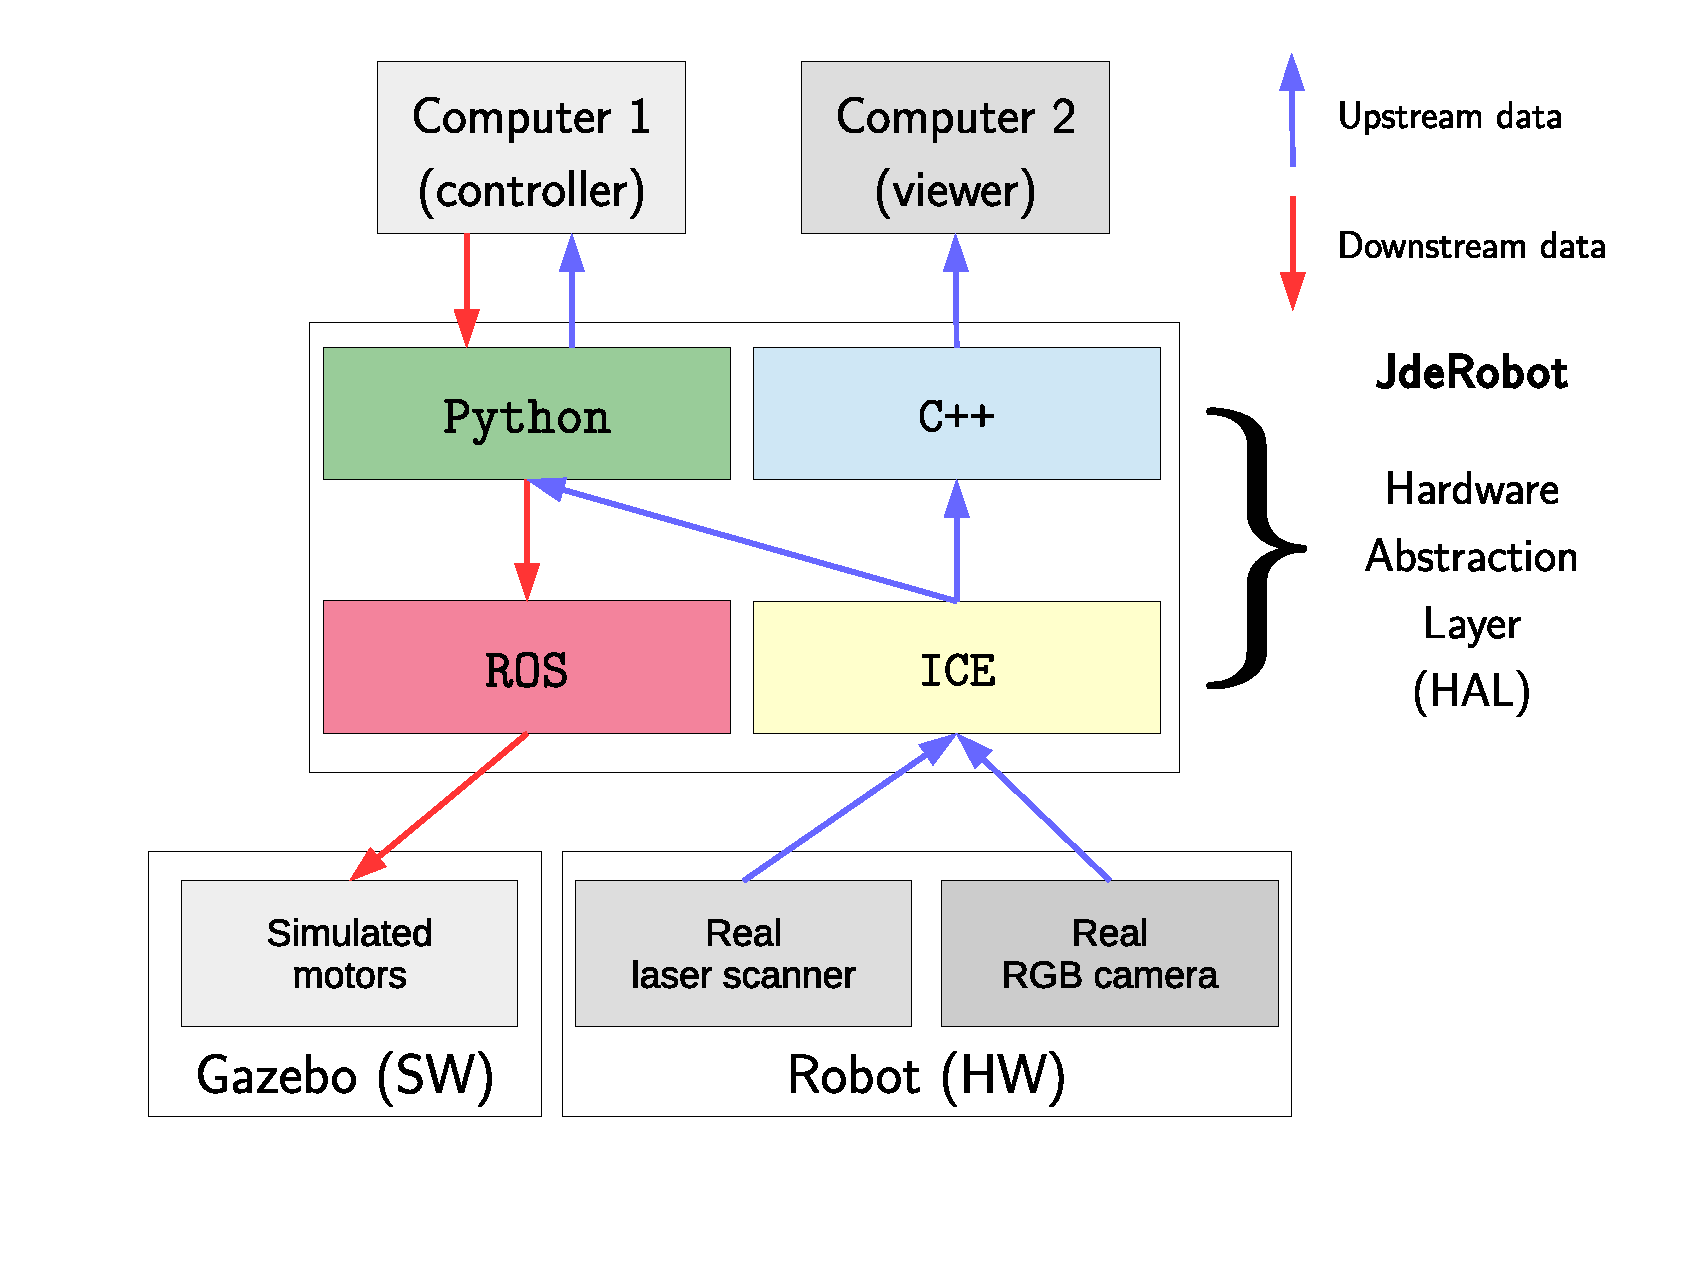
\includegraphics[width=4in]{images/jderobot_hal}
			\caption{JdeRobot abstraction layer, and a possible use distributed, multi-middleware scenario.}
			\label{fig:3_jderobot_hal}
		\end{figure}
		
.
		
		\item \textit{Wide device support:} JdeRobot provides full compatibility with ROS Kinetic Kame, so it can perfectly integrate ROS Nodes (in our concern, we can communicate with the Turtlebot and the Xtion devices via several topics that the ROS intermediate nodes open).
		
		\item \textit{Threaded software architecture for robotics applications:} as it is introduced at  \cite{jmplaza-phd}, inside a component, we will find one or more threads. These threads run concurrently with an specific timing (so it does not overload the CPU in vain if a few iterations per second are enough for a vivacious and correct response).\\
		
		These schemes perform different tasks each, on a non-blocking way, and share memory. This has been followed on a comfortable way on our implementation: the threads are independent, but the tasks they control are performed by Python objects, which are interconnected between them:
		
		
	\end{itemize}
	
	Now, in the next subsections, we will examine which of the available JdeRobot components, apart of the infrastructure, have been of greatest interest for us.
	
	\subsection{Digit Classifier node}
	\label{sec:3_digitclassifier_jderobot}
		This JdeRobot component was originally designed by David Pascual \cite{dpascualhe} and Nuria Oyaga \cite{noyaga}, and it was used on this project to land on the field of neural networks.\\
		\begin{figure}[h]
			\centering
			\includegraphics[width=4in]{images/digitclassifier}
			\caption{\texttt{DigitClassifier} on action.}
			\label{fig:3_digitclassifier}
		\end{figure}
		
		
		In rough outline, its function is to classify on-demand or in real-time the incoming images from a video source, mapping them into digits from $0$ to $9$. There are two identical version, differentiated on the underlying framework (Keras or Caffe). On \autoref{fig:3_digitclassifier} we can see its operation: it processes an image extracting the shown digit and showing the class that the network has assigned to it.\\
	
	
	\subsection{evicam\_driver driver}
	\label{sec:3_evicam_driver}
	This driver, bundled into JdeRobot\footnote{\url{https://github.com/JdeRobot/JdeRobot/tree/master/src/drivers/evicam\_driver}}, allows the user to send movements commands to a Sony EVI D100P camera \autoref{fig:3_evi}) and to retrieve information from it, creating an ICE endpoint that is ready to interact with the camera \emph{PT} (Pan, Tilt) motors.\\
	
	As this is a low-level driver, written in C++, it requires to be used on a specific way, which has been documented\footnote{\url{https://jderobot.org/Handbook\#PanTilt_Teleop}} to be easily applied in the future. This driver defines an interaction API with the camera, which allows us to get the values from the  encoders:
	\begin{lstlisting}
import config
import comm
...

cfg = config.load('yml_configuration_file')
jdrc = comm.init(cfg, 'NodeName')


# Instantiation for the motors:
PTMotors = jdrc.getPTMotorsClient('NodeName.PTMotorsEndpoint')

print(PTMotors.getLimits()) # Shows the max/min values for pan, tilt 
                            # and each speed.

print(PTMotors.motors.data) # Shows the current values for pan, tilt
                            # and each speed.

# Let's move the camera! As easy as:
PTMotors.setPTMotorsData(new_pan, new_tilt, max_pan_speed, max_tilt_speed)
	\end{lstlisting}
	
	\subsection{comm library}
		\label{sec:3_comm}
		\texttt{comm} is the basic library included on JdeRobot to perform communications between different components. It supports all the data flows in a typical scenario (\autoref{fig:3_jderobot_hal}).\\
		
		\texttt{comm} consists on a collection of bindings to easily create a link between two components, or between a device and a component. On the lowest level, we can use it relying on ROS (through topics as it was explained before on \autoref{sec:3_ros}), or through an ICE proxy. ICE\footnote{\url{https://zeroc.com/products/ice}} is an object-oriented middleware that, in our purpose, allows to abstract a data flow to a TCP/IP endpoint (an address/hostname, and a port), which can even support a communication between two or more programs inside the same machine.\\
		
		To create a communicator with \texttt{comm}, it needs the specification for that link (underlying middleware, topic/endpoint, etc.), so it uses the JdeRobot standard: YML\footnote{Legible data serialization format.} configuration files, which must follow a similar format to  \autoref{fig:3_yml_format}.
		\begin{figure}[h]
			\centering
			\includegraphics[width=4in]{images/yml_format}
			\caption{YML format required by \texttt{comm}.}
			\label{fig:3_yml_format}
		\end{figure}
		
		In the previous example (\ref{sec:3_evicam_driver}) we can see an example of an instantiation of a global communicator through \texttt{comm} (which then provides the clients to interact with the device).
		
\section{OpenCV library}
	OpenCV (\emph{Open Source Computer Vision}) is a C++/Python/Java open-source library\footnote{\url{https://opencv.org/}} (natively written in C++) for Computer Vision purposes. Among the classic/\emph{state-of-the-art} methods it bundles, we can find functions suitable for face recognition, image stitching, eye movements following, establishing markers for augmented reality, etc.\\
	
	Its general focus is \emph{efficiency and real-time functionality}, thank to low-level optimizations on the system hardware (i.e. integration with Nvidia CUDA and OpenCL GPU processing libraries). Thus, the excellent performance achieved by this open source library has turned it into the \emph{de facto} standard between every kind of users (from researchers to big companies or even governmental bodies, as their website stands).\\
	
	The main benefit we have grabbed from this library (on its version 3.3.1) has been mainly for image analysis (such as \emph{Haar Cascade} classifiers, or edge detectors) or transformations (color conversions, gaussian blurrings, etc.).\\

\section{NumPy library}
	NumPy\footnote{\url{http://www.numpy.org/}} (\emph{Numeric Python}) is a library for Python (written in C++), born to extend the numerical abilities of this language. It provides a powerful \texttt{array} class, which allows to keep a N-dimensional collection of values/objects in a really handy way (in comparison with Python's standard \emph{lists}). It also provides a rich interface to describe the arrays (such as advanced indexing, shaping, data formatting, etc.).\\
	This will such an useful resource on this work, for 3 main reasons:
	\begin{itemize}
		\item \emph{Matricial representation of images:} every processed image is handled as matrices or bigger order tensors (the concept of matrix generalized for any number of dimensions), so visualizing/slicing them becomes a trivial task.
		\item \emph{Abstract structure to keep objects:} it allows to store different objects in a \texttt{np.array} object, providing an advanced API for indexing, and conditional checks to instantly retrieve the elements fulfilling a specific condition.
		\item \emph{Saving variables into disk:} this is an useful feature for debugging purposes. \texttt{np.save()} allows to save any variable (even non-NumPy ones, like dictionaries), finding it on a \texttt{.npy} file, ready to be traced and debugged.
	\end{itemize}

In the same way than OpenCV, this is a numerical library widely adopted between Python users. This is due to the easiness of handling of its types and structures, that provides an immediate data exchange format with other parties software. It has made of it our main numerical engine on the developed purposes, having used it on its version 1.14.5.



\section{TensorFlow framework}
	\label{sec:3_tensorflow}
	TensorFlow\footnote{\url{https://www.tensorflow.org/}}, which has been the core component of this project, is an open-source software framework for high performance numerical computation. It was originally created by the Google Brain team, and it offers an excellent background for \emph{machine learning} tasks.\\
	
	Its internal functionality is based on \emph{graphs}, composed by nodes which operate and exchange data values establishing \emph{a flow of tensors} (as previously described, a tensor is the general term to describe a multidimensional structure). These tensors are handled in the backend of TensorFlow, so performing operations with tensors is really fast, in comparison with high-level mathematical libraries (NumPy). A tensor can be formed of different data types (images, words, poses, numbers, etc.), which is the key for the versatility it offers for a large variety of projects\footnote{\url{https://github.com/jtoy/awesome-tensorflow}}.\\
	
	\begin{figure}[h]
		\centering
		\includegraphics[width=4in]{images/tf_graph}
		\caption{Basic graph on TensorFlow (2 convolutional layers fed to a cost function).}
		\label{fig:3_tf_graph}
	\end{figure}
	
	All these possibilities make TensorFlow a very optimized ecosystem to implement \emph{deep learning} models (Deep Neural Networks). In addition, it is optimized for parallel GPU hardware. This gives a network the opportunity to experiment a performance boost, since it can reduce significantly the time it takes to make an inference (and even work on a system with a cluster of GPUs, although this is focused to more exigent systems than the one we create on this work). For our\\
	
	Since it was launched (November 2015), it has been adopted by many big companies which have used TensorFlow as the base for their Artificial Intelligence applications, such as Twitter, Intel, Google, eBay, Xiaomi, Nvidia, etc.\\
	
	As we will see later in the specific components, it allows to \emph{train} a neural network (for its later use) or even \emph{load} a specific model (kept on a Google Protobuf\footnote{Google's open source mechanism to serialize structured data.} \texttt{.pb} file). This is a really interesting feature, given that we are able to retrieve a bunch of pretrained models and embed them into a generic neural network.\\
	
	The version we have been using along the project is the last available one nowadays (1.9.0), compiled from sources on a Nvidia GPU (through CUDA on its 9.2.88 version), in order to squeeze the maximum inference speed possible.\\
	
	We have also also taken advantage of an included tool, \emph{TensorBoard}, which allows to \emph{visualize} interesting contents about a neural network, from a log trace of its execution. It is possible to visualize the \emph{graph} (including nodes, tensor shapes, operations, etc.). Also, it provides a functionality to analyze the obtained weights for each layer, on advanced analysis techniques, as PCA (\emph{Principal Component Analysis}). We have used it to visualize all the networks we design or import.




\section{Keras framework}
	As it is stated in \cite{dpascualhe}, Keras is a high-level \emph{neural network framework}, written in Python and capable of running on top of either TensorFlow or Theano (another \emph{deep learning} library).\\
	
	Hence, it is an abstraction with the goal of programming and handling a neural network on an simpler way, relying on a powerful library (treated as \emph{backend}) as TensorFlow to perform all the numeric operations. As well as TensorFlow, it is capable of loading previously compiled and saved models, on the serialization standard HDF5\footnote{Hierarchical Data Format (v.5): general purpose format to store and manage data.} (\texttt{.h5} files).\\
	
	In our project, support has been provided to use this framework (selecting it on the YML configuration file) on its version 2.2.0, although our main interest has been TensorFlow due to the significative difference of processing speed between both frameworks (being TensorFlow twice as fast as Keras).
\section{PyQt framework}
	Qt\footnote{\url{https://www.qt.io/}} is an cross-platform object-oriented framework for building GUIs (\emph{Graphical User Interfaces}), originally developed by a Nokia department. It is distributed under a commercial license, although it has a standard GPL license for open-source projects.\\
	
	A third party company (RiverBank Computing) developed PyQt, a set of Python bindings to interact with Qt (originally written in C++). It is structured in units called \emph{Widgets}, which contain blocks (\emph{Labels}).\\
	
	All this allows to easily deploy a GUI-based(\emph{Graphic User Interface}) program:
	\begin{figure}[h]
		\centering
		\begin{subfigure}[h]{0.55\linewidth}
			\centering
			\begin{lstlisting}
import sys
from PyQt5 import QtGui, QtWidgets

def window():
	app = QtWidgets.QApplication(sys.argv)
	w = QtWidgets.QWidget()
	b = QtWidgets.QLabel(w)
	b.setText("Hello World!")
	w.setGeometry(100,100,200,50)
	b.move(50,20)
	w.setWindowTitle("PyQt")
	w.show()
	sys.exit(app.exec_())

if __name__ == '__main__':
	window()
			\end{lstlisting}
			\caption{\emph{Hello world} example code.}
		\end{subfigure}
		\qquad
		\begin{subfigure}[h]{0.35\linewidth}
			\centering
			\includegraphics[width=3in]{images/pyqt_helloworld}
			\caption{Resulting window.}
		\end{subfigure}
		\caption{Example of a \emph{Hello World} window with PyQt5 bindings.}
		\label{fig:3_pyqt_helloworld}
	\end{figure}
	
	As it is the last available version at the time this is developed, we have used the version 5 of Qt. Hence, our binding library is \texttt{PyQt5}, which has been used to build a live-capable GUI on an intuitive way, in all the developed tools.\\
	
\section{threading library}
	\label{sec:3_threading}
	\texttt{Threading}\footnote{\url{https://docs.python.org/2/library/threading.html}} is a Python standard library which offer a high-level API for threading processes. This means to run programs on more than one single job for the CPU, which allows to be capable of perform several tasks on a simultaneous way.\\
	
	This is very convenient for our purpose, as we want to stick to a multiprocessing paradigm. So, this way we can have dedicated threads to grab the new camera images, update the GUI, and make the Neural Network to load new inferences on the last image detected.\\
	
	The \texttt{threading} provides a generic class for a thread. Our only task is to create a custom class which inherits it, customizing the \texttt{\_\_init\_\_} and \texttt{run()} methods our own way:
	

	\begin{lstlisting}
...
import threading
from datetime import datetime
...

class MyThread(threading.Thread):

	def __init__(self, foo, bar):
		'''
		This is the method which will be called at the creation of the thread.
		'''
		self.my_foo = foo
		self.my_bar = bar
		self.time_cycle = 100 # ms
		threading.Thread.__init__(self)  # Rest of the initialization.
		
		
	def run(self):
		'''
		This is the task the thread will perform once.
		If we put an infinite loop inside, we have a periodic thread.
		'''
		while True:
			start_time = datetime.now()
			# Grab an image, or run an inference on the neural network...
			self.my_foo.doMyStuff(self.my_bar)
			end_time = datetime.now()
			dt = end_time - start_time
			
			# If it did not take the refresh time, it sleeps until it arrives.
			if dt < self.t_cycle:
				sleep(self.t_cycle - dt)
				
	\end{lstlisting}
	
In addition, as we can see, it is possible to control the update period of the thread, so we can decide how much time it will be elapsed between two consecutive executions of the thread task (and of course this is a tunable parameter).\\

The version we have used is the standard one included with the Python installation.

	
	\chapter{\texttt{ObjectDetector} node}
\section{Description}
\section{Functional architecture}
\section{Neural Network processing}


\chapter{\texttt{FollowPerson} node}
\label{chap:followperson}
\section{Description}
	\subsection{First approach: PTZ Camera}
	\label{sec:follow_ptz}
	\subsection{Second approach: Turtlebot/Xtion set}
	\label{sec:follow_turtlebot}
\section{Functional architecture}
\section{Neural Network processing}
\section{Face detection and identification}
\section{Tracking algorithm}
\section{Physical response (\emph{PID} controller)}



\chapter{Conclusions}
	\section{Conclusions}
	\section{Future research lines}
	
	
	%%%%%%%%% BIBLIOGRAPHY %%%%%%%%%
	\section{Bibliography}
	\bibliography{bibliography}
	\bibliographystyle{unsrt}
\end{document}